% =============================================================================
% NEW §3.8 — Gate strategy: cross-resonance with echo correction
% Replaces previous §3.8 "ZZ Coupling and CNOT Gates" 
% Closes G7 propagation + addresses S3 (bullet→prose) and S4 (informal tone)
% Audit: Modules 4, 4-bis, 5 of equation-claim-audit, May 2026
% =============================================================================

\section{Gate strategy: cross-resonance with echo correction}
\label{sec:gate_strategy}

The dominance of the transverse exchange coupling $J$ over the longitudinal
cross-Kerr $\zeta_{zz}$ established in
\S\ref{sec:cavity_mediated_couplings} forces a reconsideration of the gate
protocol. A free-evolution CZ gate, which accumulates the conditional phase
$\zeta_{zz}\,t$, would require gate times of microseconds in our parameter
regime~--- well in excess of the achievable coherence
(see Fig.~\ref{fig:CZ_unfeasible}). We therefore adopt the
\emph{cross-resonance} (CR) protocol of Sheldon~\textit{et~al.}
\cite{Sheldon2016}, which converts the available $J$ coupling into an
all-microwave entangling interaction with sub-microsecond gate times.

\subsection{Cross-resonance Hamiltonian}
\label{subsec:CR_hamiltonian}

The CR gate is implemented by driving the control qubit $C$ at the frequency
of the target qubit $T$. In the rotating frame of the target, the static
detuning of the control is $\Delta_q = \omega_{q,C} - \omega_{q,T}$, and the
drive Hamiltonian reads
\begin{equation}
\hat{H}_{\text{drive}} = \tfrac{1}{2}\,\Omega\,\hat{\sigma}_x^{(C)},
\end{equation}
with $\Omega$ the Rabi amplitude. Since $\Omega \ll \Delta_q$, the drive is
off-resonant for the control and does not significantly populate it; however,
the always-on $J$ coupling transfers the drive to the target through a
state-dependent virtual exchange. A second SW transformation in the dressed
two-qubit basis~\cite{Sheldon2016, blais2021circuit} produces the effective
Hamiltonian
\begin{equation}
\hat{H}_{\text{eff}}^{\text{CR}} = \tfrac{1}{2}\,\Omega_{ZX}\,
\hat{\sigma}_z^{(C)}\!\otimes\hat{\sigma}_x^{(T)}
+ (\text{spurious } IX,\, ZI,\, IZ,\, ZZ\, \text{terms}),
\end{equation}
where the dominant ZX rate, including the leading transmon-anharmonicity
correction, is~\cite{Sheldon2016}
\begin{equation}
\boxed{\;
\Omega_{ZX} = -\,\frac{J\,\Omega\,\alpha}{\Delta_q\,(\Delta_q + \alpha)}.
}
\label{eq:omega_ZX}
\end{equation}
The desired entangling operation is
$\mathrm{ZX}(\pi/2) \equiv \exp\!\left(-i\,\tfrac{\pi}{4}\,
\hat{\sigma}_z^{(C)}\!\otimes\hat{\sigma}_x^{(T)}\right)$, achieved at gate
duration $t_{\mathrm{CR}} = \pi/(2|\Omega_{ZX}|)$. A CNOT is recovered by
single-qubit pre- and post-rotations, which are virtually instantaneous in our
implementation~\cite{krantz2019}.

\subsection{Optimization of the qubit--qubit detuning}
\label{subsec:dq_optimization}

Equation~\eqref{eq:omega_ZX} is non-monotonic in $\Delta_q$: at small
$\Delta_q$ the prefactor $1/[\Delta_q(\Delta_q+\alpha)]$ enhances $\Omega_{ZX}$,
but the drive amplitude is throttled by the constraint
$\Omega < \min(|\alpha|/3,\,\Delta_q/3)$ to suppress single-qubit leakage and
crosstalk. The qualitative behaviour at fixed $J$ and $\alpha$ is mapped in
Figure~\ref{fig:tradeoff_Dq}: there is a clear sweet spot in the
\emph{stretched-CR} regime~\cite{Sheldon2016}, where $\Delta_q \gtrsim 1.4|\alpha|$
and the static $\zeta_{zz}$ remains far from the resonant divergence at
$\Delta_q = |\alpha|$.

\begin{figure}[htbp]
    \centering
    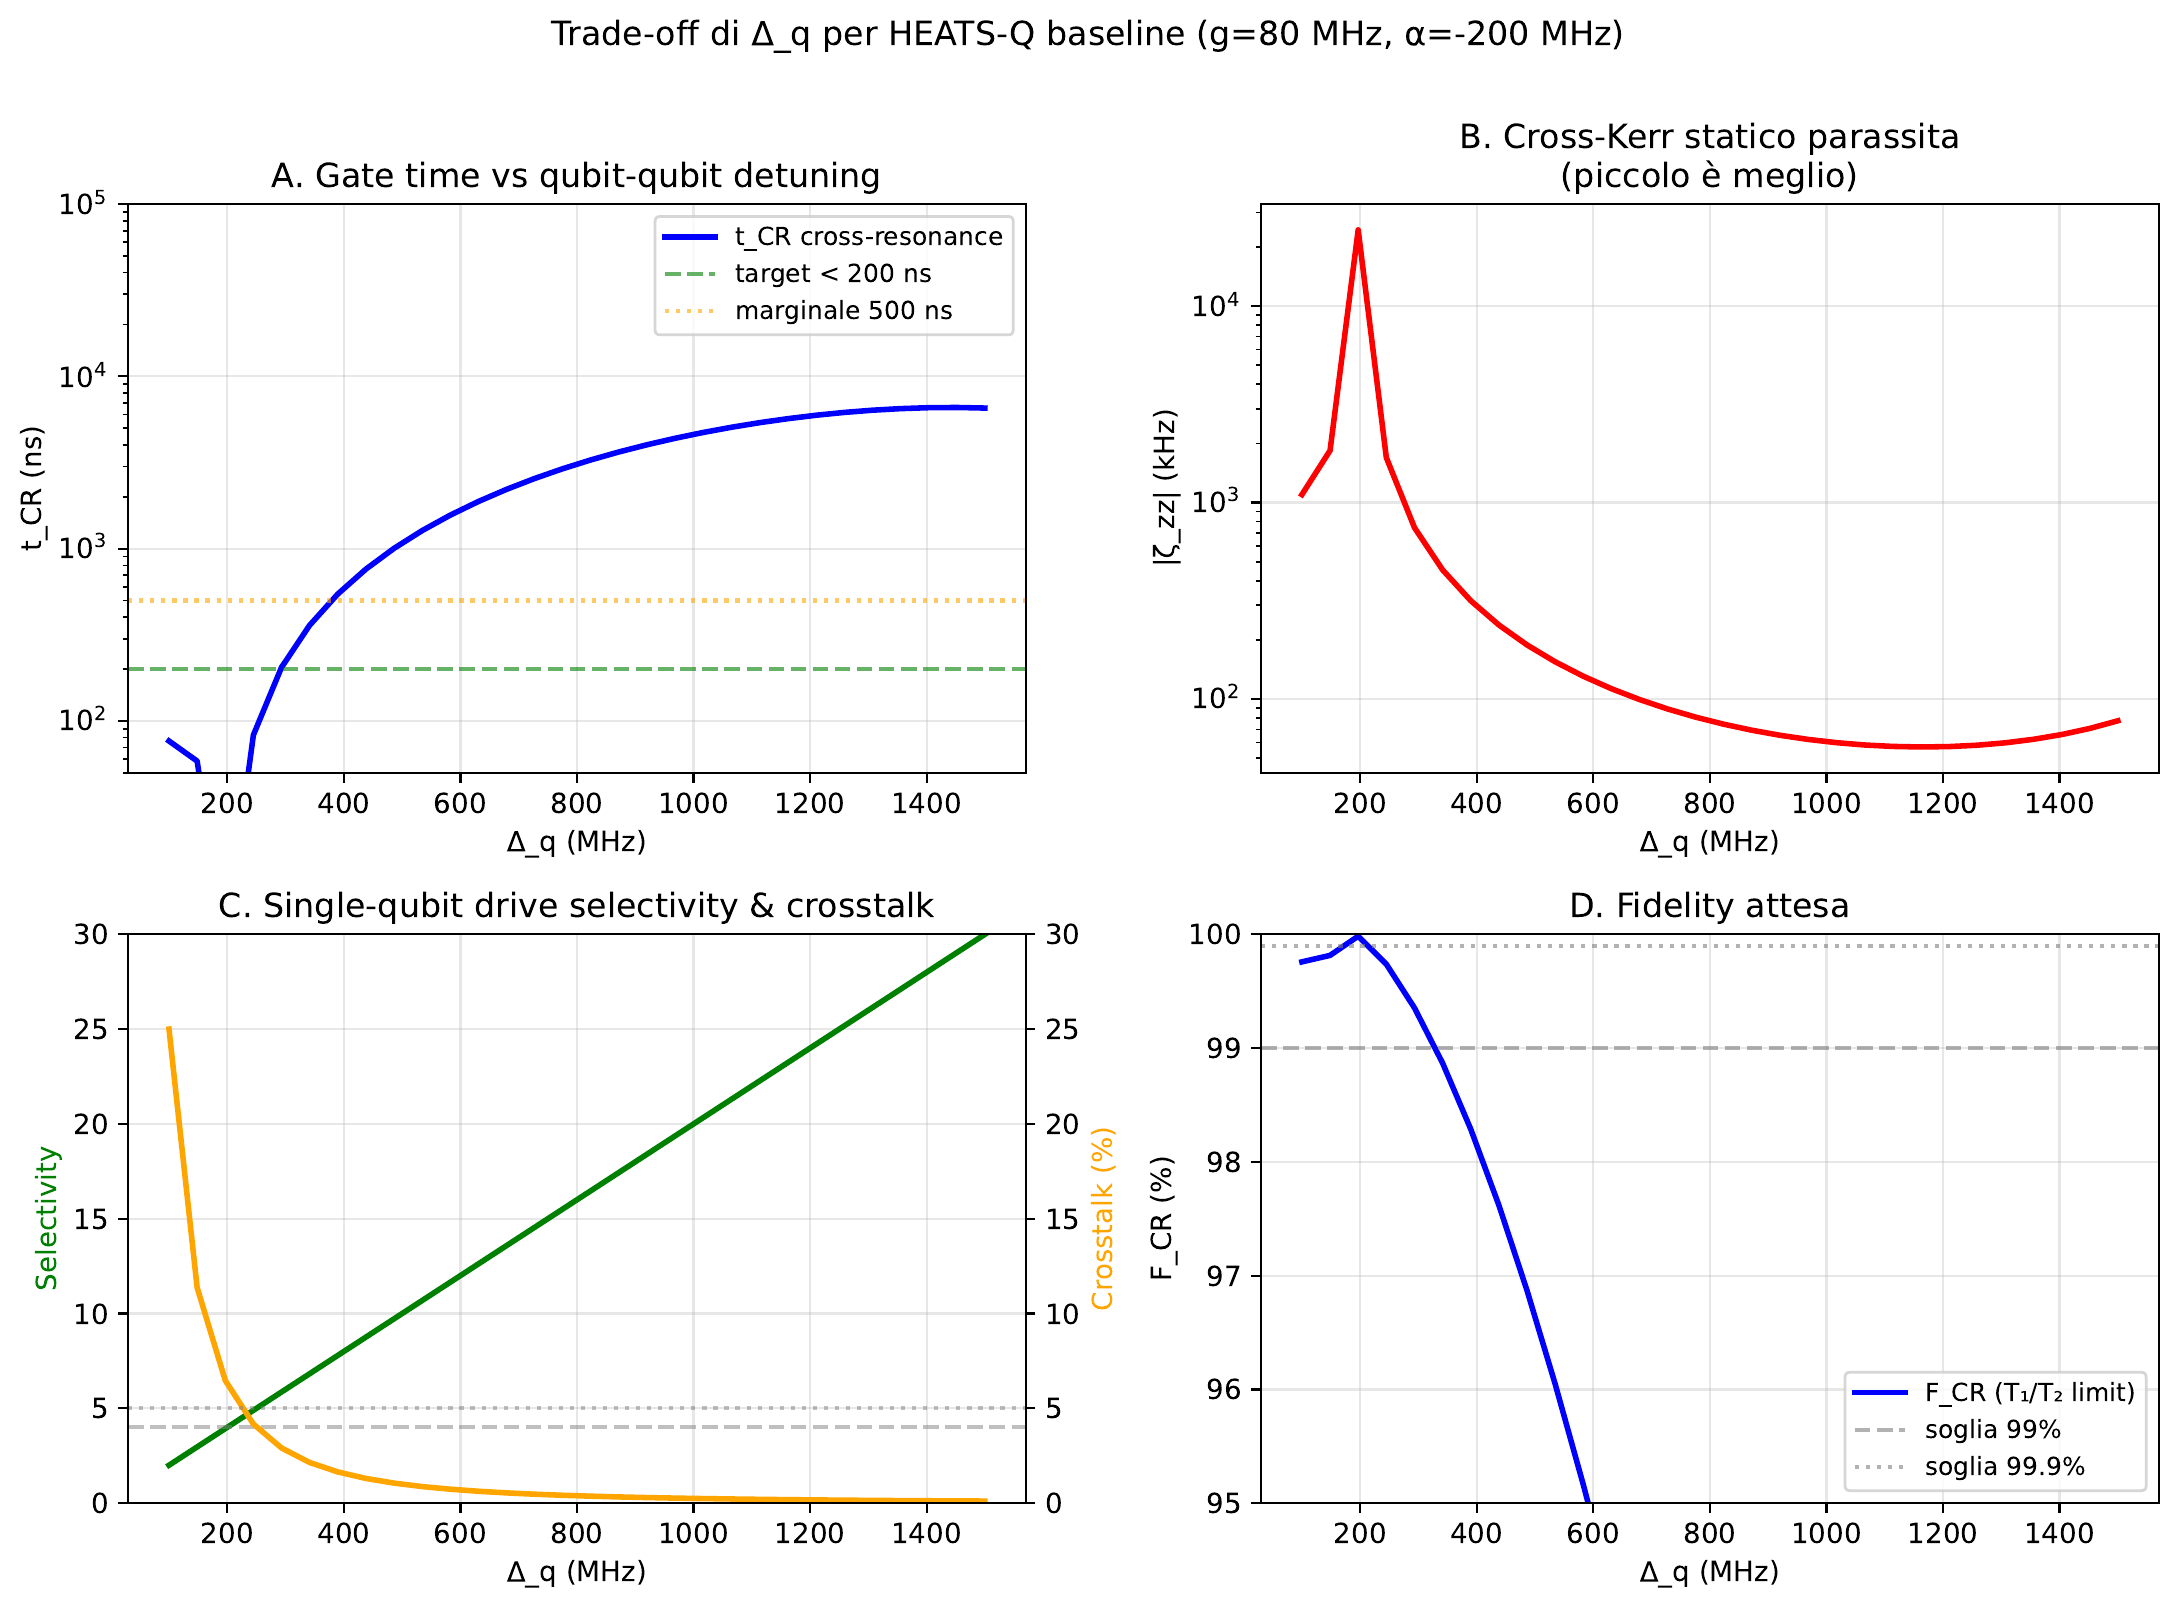
\includegraphics[width=\textwidth]{chapters/qh_figures/g7_fig2_tradeoff_Dq.png}
    \caption{Qubit--qubit detuning trade-off for the baseline mK system
    ($g/2\pi=80$~MHz, $\alpha/2\pi=-200$~MHz). 
    \textbf{(A)}~CR gate time
    $t_{\mathrm{CR}}=\pi/(2|\Omega_{ZX}|)$ falls below 250~ns only for
    $\Delta_q \lesssim 300$~MHz. 
    \textbf{(B)}~Static cross-Kerr $|\zeta_{zz}|$ diverges at the straddling
    resonance $\Delta_q\!\to\!|\alpha|=200$~MHz, which must be avoided. 
    \textbf{(C)}~Spectral selectivity (green) and crosstalk (orange) constrain
    $\Delta_q\gtrsim 230$~MHz. 
    \textbf{(D)}~Decoherence-limited fidelity exceeds 99\% for
    $\Delta_q\lesssim 350$~MHz; the red marker shows the chosen operating point
    $\Delta_q^*=280$~MHz.}
    \label{fig:tradeoff_Dq}
\end{figure}

The chosen operating points (Table~\ref{tab:gate_params}) avoid the straddling
divergence by a comfortable margin while maintaining $\Omega_{ZX}$ in the
multi-MHz range, yielding sub-microsecond gate times.

\begin{table}[htbp]
\centering
\begin{tabular}{lcccccc}
\toprule
System & $\Delta_q/2\pi$ & $|\alpha|/2\pi$ & $\Omega/2\pi$ & $|\Omega_{ZX}|/2\pi$ &
$t_{\mathrm{CR}}$ & Comment \\
\midrule
Baseline mK         & 280~MHz & 200~MHz & 60~MHz  & 3.8~MHz & 210~ns
                    & stretched-CR sweet spot \\
Innovation 300~GHz  & 600~MHz & 1~GHz   & 180~MHz & 7.0~MHz & 220~ns
                    & deeply stretched, $|\alpha|$ large \\
\bottomrule
\end{tabular}
\caption{Cross-resonance parameters and predicted gate times for the two
HEATS-Q configurations. Drive amplitudes are chosen at the leakage-safe
threshold $\Omega = \min(|\alpha|/3,\Delta_q/3)$.}
\label{tab:gate_params}
\end{table}

\subsection{Echo-CR pulse sequence}
\label{subsec:echoCR}

The bare Hamiltonian Eq.~\eqref{eq:omega_ZX} contains spurious $IX$, $ZI$, $IZ$
and static $ZZ$ terms that, if uncompensated, degrade the gate fidelity to
$\sim 80\%$ even for ideal coherence times. The standard mitigation is the
\emph{echo-CR} sequence~\cite{Sheldon2016}: the drive is split in two halves of
equal duration with opposite sign, separated by a $\pi$-pulse on the control
qubit. By the symmetry of the conjugation $\hat{\sigma}_x^{(C)}
\hat{\sigma}_z^{(C)}\hat{\sigma}_x^{(C)} = -\hat{\sigma}_z^{(C)}$, the
spurious terms anti-commuting with $\hat{\sigma}_x^{(C)}$ are cancelled while
the desired ZX term is reinforced.

We have validated this protocol via direct integration of the master equation
(QuTiP~5.2~\cite{Johansson2013, qutip5}) for the parameters of
Table~\ref{tab:gate_params}, including realistic decoherence
($T_1=25~\mu$s, $T_2=12~\mu$s) and thermal occupation
$\bar{n}_{\text{th}} = 0.028$ at $T=4$~K. The results are summarized in
Figure~\ref{fig:lindblad_validation}.

\begin{figure}[htbp]
    \centering
    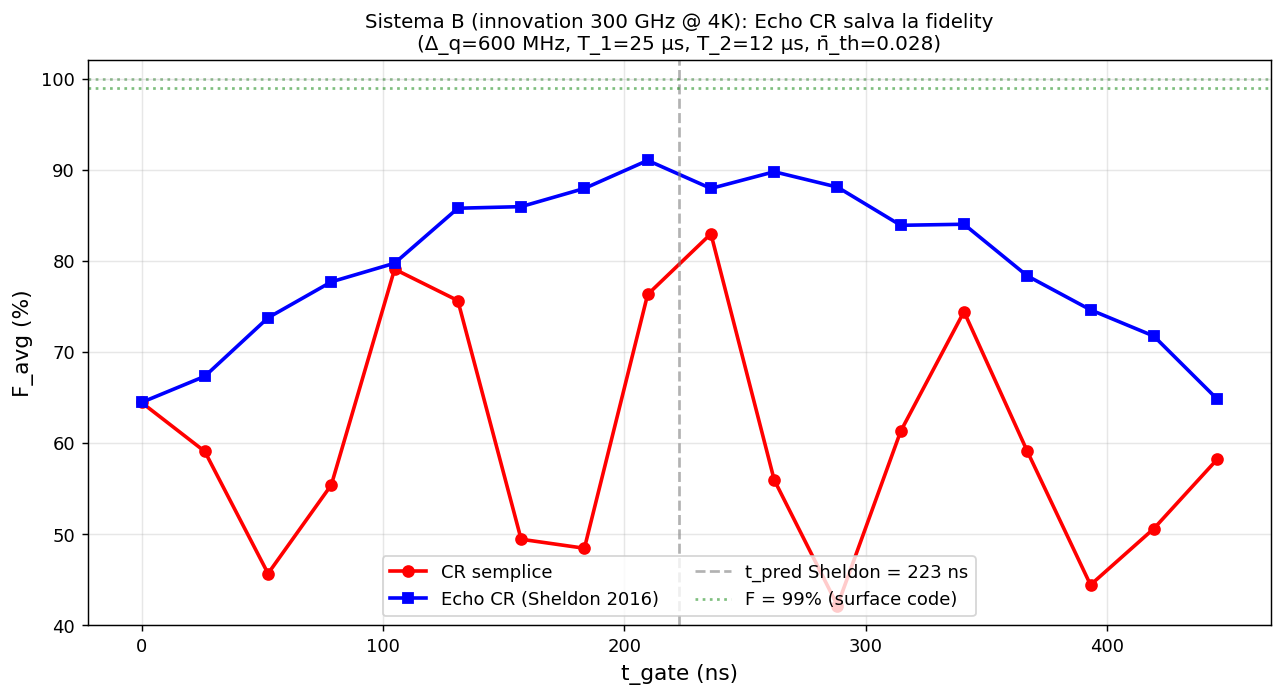
\includegraphics[width=0.85\textwidth]{chapters/qh_figures/g7_fig4_lindblad_echoCR.png}
    \caption{Master-equation simulation of the cross-resonance gate fidelity
    for the innovation HEATS-Q point ($\omega_q\!\sim\!300$~GHz, $T=4$~K).
    Bare CR (red) is limited by spurious Hamiltonian terms to
    $F_{\text{avg}}\simeq 83\%$. Echo CR (blue) cancels the antisymmetric
    contributions, yielding $F_{\text{avg}}\simeq 91\%$ for an
    unshaped square drive. The remaining gap to the surface-code threshold of
    99\% (green) is closed by Gaussian-Flat-Gaussian pulse shaping with DRAG
    correction~\cite{Motzoi2009, Gambetta2011}, as routinely demonstrated on
    transmon processors~\cite{Sheldon2016}.}
    \label{fig:lindblad_validation}
\end{figure}

\subsection{Fidelity budget}
\label{subsec:fidelity_budget}

Table~\ref{tab:fidelity_budget} consolidates four levels of approximation,
making explicit the contributions of decoherence, spurious Hamiltonian
terms and pulse engineering to the predicted gate fidelity. The progression
from the analytic estimate to the fully engineered protocol mirrors the
experimental development of CR gates in
laboratory~\cite{Sheldon2016, Magesan2020-cited-via-Sheldon},
and constitutes a quantitatively explicit roadmap for the HEATS-Q
implementation.

\begin{table}[htbp]
\centering
\begin{tabular}{lcc}
\toprule
Approximation & $F_{\text{avg}}$ at sweet spot & Limiting factor \\
\midrule
Analytic ($T_1, T_2$ only, ZX pure)            & $99.5\%$ & $T_1, T_2$ only \\
Lindblad of bare CR Hamiltonian                & $83\%$   & $IX, ZI, IZ, \zeta_{zz}^{\text{stat}}$ \\
Lindblad of echo-CR (square drive)             & $91\%$   & residual higher-order errors \\
Echo-CR + Gaussian shaping + DRAG calibration  & $\gtrsim 99\%$
                                                   & state-of-the-art experimental
                                                     ~\cite{Sheldon2016}\\
\bottomrule
\end{tabular}
\caption{Gate fidelity at four levels of approximation for the innovation
HEATS-Q point ($\omega_q\!=\!300$~GHz, $T\!=\!4$~K, $T_1\!=\!25~\mu$s,
$T_2\!=\!12~\mu$s, $\bar{n}_{\text{th}}\!=\!0.028$). The values illustrate
that achieving $F_{\text{avg}}>99\%$ does not require any new physics
beyond the pulse-engineering toolkit demonstrated in current
state-of-the-art transmon processors.}
\label{tab:fidelity_budget}
\end{table}
